%! Author = ben
%! Date = 24.10.2023

\documentclass[./entry.tex]{subfiles}
\usepackage{biblatex}
\usepackage{multirow}
\usepackage{colortbl}

\begin{document}

    In der Informatik wird die Laufzeit eines Algorithmus in der Regel in der sogenannten \dq Big-O-Notation\dq\ angegeben.
    Im Beispiel $O(n)$ geht man von einer linearen Laufzeit aus, das heißt, dass die Anzahl der
    Vergleiche proportional zur Anzahl der Elemente ist.
    \dq$n$\dq\ steht hierbei für die Anzahl der Elemente in der zu sortierenden Datenmenge.
    In der Tabelle \ref{tab:runtimeanalysis} sind die Laufzeiten der benannten Sortieralgorithmen aufgelistet.\footnote{\bscite{big-o-notation}}


    \begin{table}[h]
        \centering
        \begin{tabular}{|c|c|c|c|}
            \hline
            \textbf{Algorithmus}                                                     & \textbf{bester Fall} & \textbf{schlechtester Fall} & \textbf{Durchschnitt} \\
            \hline
            \textbf{BubbleSort}\tablefootnote{\bscite{bubble-sort-aufwand}}          & $O(n)$               & $O(n^2)$                    & $O(n^2)$             \\
            \hline
            \textbf{SelectionSort}\tablefootnote{\bscite{selection-sort-complexity}} & $O(n)$               & $O(n^2)$ & $O(n^2)$ \\
            \hline
            \textbf{InsertionSort}\tablefootnote{\bscite{insertion-sort}}            & $O(n)$               & $O(n^2)$                    & $O(n^2)$             \\
            \hline
            \textbf{QuickSort}\tablefootnote{\bscite{quick-sort}}                    & $O(n \times log(n))$ & $O(n^2)$                    & $O(n \times log(n))$             \\
            \hline
        \end{tabular}
        \caption{Laufzeit-/Aufwandsanalyse der Sortieralgorithmen}
        \label{tab:runtimeanalysis}
    \end{table}

    \paragraph{Visualisierung} Die \dq Big-O-Notation\dq\ kann auch grafisch dargestellt werden.
    Hierbei wird die Anzahl der zu sortierenden Elemente auf der $x$-Achse und die Anzahl der Vergleiche auf der $y$-Achse aufgetragen:


    \begin{multicols}{3}

        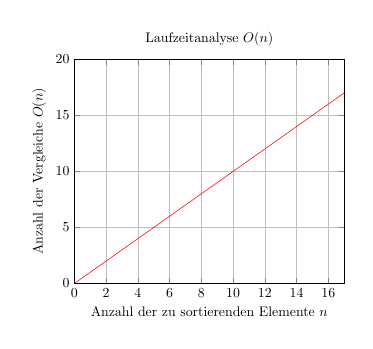
\begin{tikzpicture}[scale=0.5]
            \begin{axis}
                [
                title={Laufzeitanalyse $O(n)$},
                xlabel={Anzahl der zu sortierenden Elemente $n$},
                ylabel={Anzahl der Vergleiche $O(n)$},
                grid,
                xmin=0,
                xmax=17,
                ymin=0,
                ymax=20
                ]

                \addplot[domain=0:17, color=red]{x};
            \end{axis}
        \end{tikzpicture}

        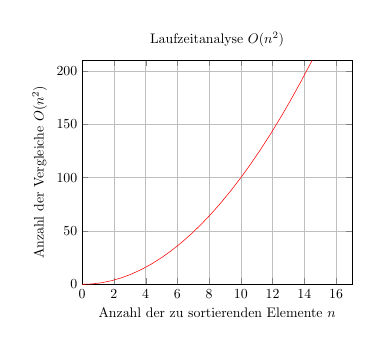
\begin{tikzpicture}[scale=0.5]
            \begin{axis}
                [
                title={Laufzeitanalyse $O(n^2)$},
                xlabel={Anzahl der zu sortierenden Elemente $n$},
                ylabel={Anzahl der Vergleiche $O(n^2)$},
                grid,
                xmin=0,
                xmax=17,
                ymin=0,
                ymax=210
                ]

                \addplot[domain=0:15, color=red]{x^2};
            \end{axis}
        \end{tikzpicture}


        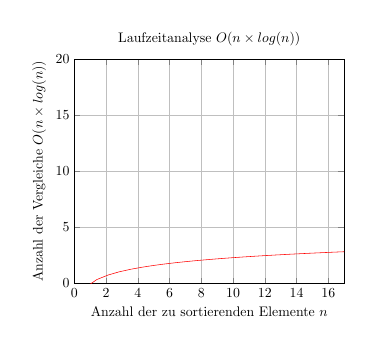
\begin{tikzpicture}[scale=0.5]
            \begin{axis}
                [
                title={Laufzeitanalyse $O(n \times log(n))$},
                xlabel={Anzahl der zu sortierenden Elemente $n$},
                ylabel={Anzahl der Vergleiche $O(n \times log(n))$},
                grid,
                xmin=0,
                xmax=17,
                ymin=0,
                ymax=20
                ]

                \addplot[domain=0:17, color=red]{ln(x)};
            \end{axis}
        \end{tikzpicture}
    \end{multicols}

    \paragraph{Auswertung}
    Man kann erkennen, dass sowohl der BubbleSort-Algorithmus als auch der SelectionSort-Algorithmus
    und der InsertionSort-Algorithmus im Durchschnitt eine quadratische Laufzeit haben, was bei allen
    drei Algorithmen dem schlechtesten Fall entspricht.
    Vergleicht man nun diese Algorithmen mit dem QuickSort-Algorithmus, so fällt auf, dass dieser
    im Durchschnitt eine deutlich geringere Laufzeit hat und somit effizienter arbeitet.
    Dies liegt daran, dass der QuickSort-Algorithmus die Datenmenge in jedem Schritt halbiert,
    wodurch die Anzahl der Vergleiche deutlich geringer ist.
    Der QuickSort-Algorithmus hat allerdings auch einen schlechtesten Fall, in dem er eine quadratische Laufzeit hat.
    Dieser Fall tritt ein, wenn die Datenmenge bereits sortiert ist und das Pivot-Element immer das kleinste oder größte Element ist.
\end{document}